\begin{tikzpicture}[x=1cm, y=1cm, font=\sffamily\footnotesize,
  ptitle/.style={anchor=west, font=\sffamily\bfseries\small, text=narrareddeep},
  textbox/.style={draw=phaseA!60, fill=phaseA!6, rounded corners=2pt, inner sep=4pt, anchor=north west,
                  align=left, font=\sffamily\scriptsize},
  lbl/.style={draw=#1, fill=white, fill opacity=0.9, text opacity=1, rounded corners=1pt, inner sep=1.6pt,
              line width=0.6pt, font=\sffamily\scriptsize},
  lblkey/.style={draw=#1, fill=white, fill opacity=0.95, text opacity=1, rounded corners=1pt, inner sep=1.8pt,
                 line width=1.0pt, font=\sffamily\scriptsize\bfseries},
  lead/.style={draw=#1, line width=0.7pt},
  path/.style={-{Latex[length=2.6mm, width=2.4mm]}, draw=black!85, line width=1.6pt},
  imgcap/.style={anchor=north, font=\sffamily\scriptsize, text=black!60},
  chip/.style={draw=black!30, fill=white, rounded corners=6pt, inner sep=2.5pt, font=\sffamily\footnotesize},
  flow/.style={-{Latex[length=1.6mm]}, draw=black!50, line width=0.6pt},
  lab/.style={anchor=east, font=\sffamily\footnotesize, text=black!75},
  txt/.style={anchor=west, font=\sffamily\footnotesize, text=black!75}]

\node[ptitle] at (0,0.000) {(a) An example task of this family and its room (AI2-THOR rendering)};
\node[textbox, text width=14.70cm] (obs) at (0,-0.280) {\textbf{Goal.} Your task is to: put a clean soapbar in countertop.\\[1pt]\textbf{Initial observation.} You are in the middle of a room. Looking quickly around you, you see a cabinet 4, a cabinet 3, a cabinet 2, a cabinet 1, a countertop 1, a garbagecan 1, a handtowelholder 2, a handtowelholder 1, a sinkbasin 2, a sinkbasin 1, a toilet 1, a toiletpaperhanger 1, and a towelholder 1.};
\begin{scope}[shift={($(obs.south west)+(0,-0.25)$)}]
\node[anchor=north west, inner sep=0] at (0.000,0.000) {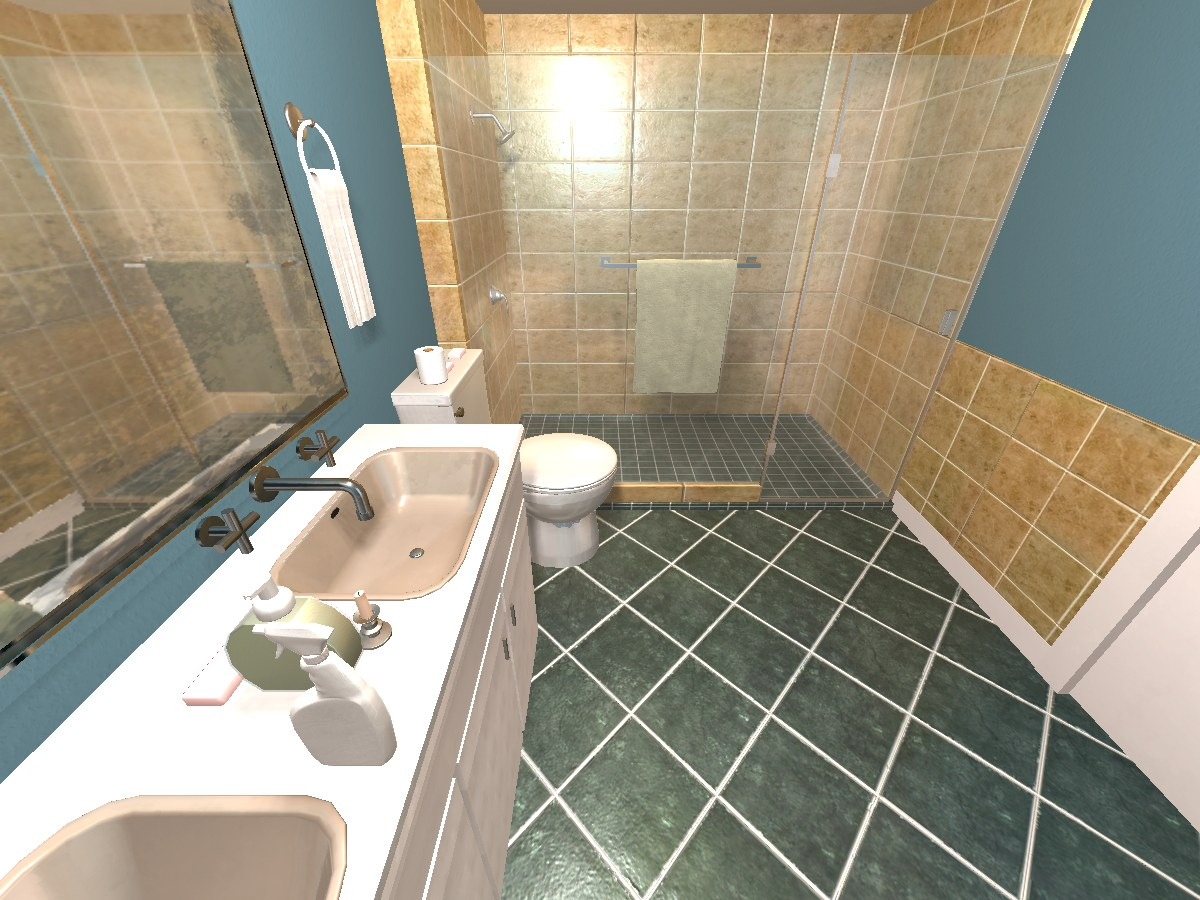
\includegraphics[width=9.012cm]{figures/cases/clean_view1.jpg}};
\draw[black!35, line width=0.4pt] (0.000,0.000) rectangle ++(9.012,-6.759);
\draw[dimF, line width=1.1pt] (3.428,-2.658) circle (0.160);
\draw[lead=dimF] (3.428,-2.658) -- (3.428,-2.158);
\fill[dimF] (3.428,-2.658) circle (0.06);
\node[lblkey=dimF] at (3.428,-2.158) {soapbar};
\draw[dimE, line width=1.1pt, rounded corners=1pt] (0.000,-5.978) rectangle (2.598,-6.759);
\draw[lead=dimE] (1.299,-6.368) -- (3.315,-6.368);
\fill[dimE] (1.299,-6.368) circle (0.06);
\node[lblkey=dimE] at (3.315,-6.368) {sinkbasin: clean it here};
\draw[liftpositive, line width=1.1pt, rounded corners=1pt] (0.000,-3.192) rectangle (3.905,-6.759);
\fill[liftpositive] (1.953,-4.975) circle (0.06);
\node[lblkey=liftpositive] at (1.953,-4.975) {countertop: put it here};
\draw[dimA, line width=1.1pt, rounded corners=1pt] (2.936,-2.628) rectangle (4.634,-4.266);
\draw[lead=dimA] (3.785,-3.447) -- (3.785,-2.947);
\fill[dimA] (3.785,-3.447) circle (0.06);
\node[lblkey=dimA] at (3.785,-2.947) {toilet: the soapbar is here};
\draw[lead=black!55] (2.880,-3.935) -- (2.880,-3.435);
\fill[black!55] (2.880,-3.935) circle (0.06);
\node[lbl=black!45] at (2.880,-3.435) {sinkbasin};
\draw[lead=black!55] (3.665,-5.610) -- (2.715,-5.418);
\fill[black!55] (3.665,-5.610) circle (0.06);
\node[lbl=black!45] at (2.715,-5.418) {cabinets};
\node[anchor=north west, inner sep=0] at (9.262,0.000) {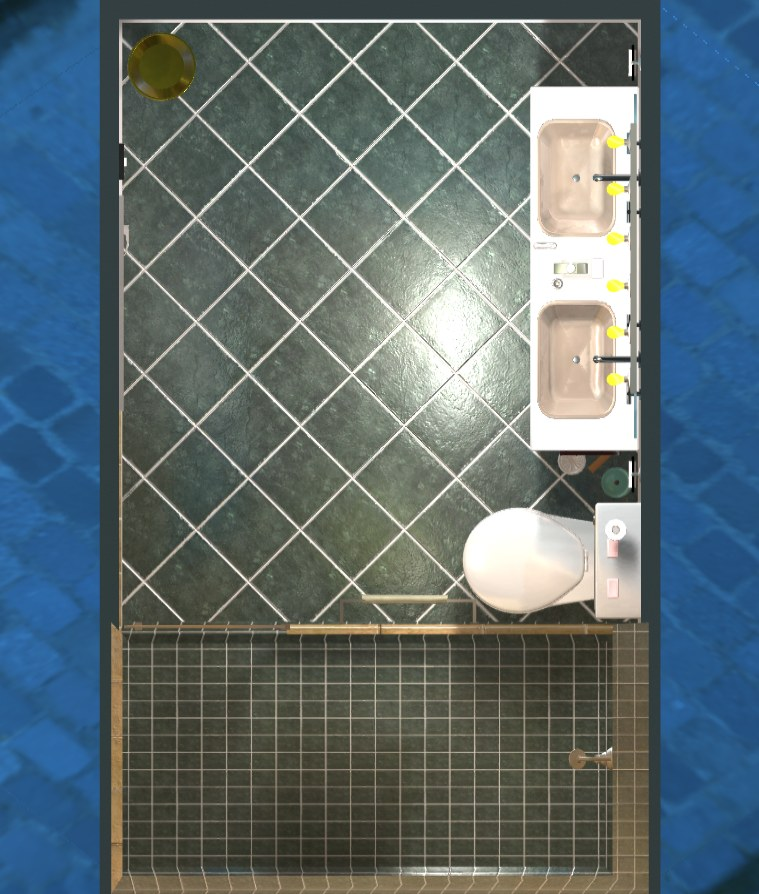
\includegraphics[width=5.738cm]{figures/cases/clean_map.jpg}};
\draw[black!35, line width=0.4pt] (9.262,0.000) rectangle ++(5.738,-6.759);
\fill[black, opacity=0.22] (12.888,-1.368) -- ++(-135:1.1) arc (-135:-45:1.1) -- cycle;
\fill[black] (12.888,-1.368) circle (0.08);
\draw[white, line width=3.4pt, opacity=0.85] (13.251,-4.028) -- (13.577,-1.589);
\draw[path] (13.251,-4.028) -- (13.577,-1.589);
\draw[white, line width=3.4pt, opacity=0.85] (13.631,-1.540) -- (13.656,-1.782);
\draw[path] (13.631,-1.540) -- (13.656,-1.782);
\draw[lead=dimA] (13.225,-4.226) -- (13.225,-3.726);
\fill[dimA] (13.225,-4.226) circle (0.06);
\node[lblkey=dimA] at (13.225,-3.726) {toilet: the soapbar is here};
\draw[lead=dimE] (13.610,-1.341) -- (13.197,-0.879);
\fill[dimE] (13.610,-1.341) circle (0.06);
\node[lblkey=dimE] at (13.197,-0.879) {sinkbasin: clean it here};
\draw[lead=liftpositive] (13.682,-2.031) -- (11.977,-1.839);
\fill[liftpositive] (13.682,-2.031) circle (0.06);
\node[lblkey=liftpositive] at (11.977,-1.839) {countertop: put it here};
\draw[lead=black!55] (13.305,-2.015) -- (12.665,-2.368);
\fill[black!55] (13.305,-2.015) circle (0.06);
\node[lbl=black!45] at (12.665,-2.368) {cabinets};
\draw[lead=black!55] (10.484,-0.503) -- (10.192,-0.965);
\fill[black!55] (10.484,-0.503) circle (0.06);
\node[lbl=black!45] at (10.192,-0.965) {garbagecan};
\draw[lead=black!55] (14.109,-3.587) -- (13.773,-3.125);
\fill[black!55] (14.109,-3.587) circle (0.06);
\node[lbl=black!45] at (13.773,-3.125) {handtowelholder};
\draw[lead=black!55] (14.109,-0.475) -- (12.806,-0.283);
\fill[black!55] (14.109,-0.475) circle (0.06);
\node[lbl=black!45] at (12.806,-0.283) {handtowelholder};
\draw[lead=black!55] (13.610,-2.715) -- (14.279,-2.361);
\fill[black!55] (13.610,-2.715) circle (0.06);
\node[lbl=black!45] at (14.279,-2.361) {sinkbasin};
\draw[lead=black!55] (13.675,-3.332) -- (13.675,-4.132);
\fill[black!55] (13.675,-3.332) circle (0.06);
\node[lbl=black!45] at (13.675,-4.132) {toiletpaperhanger};
\draw[lead=black!55] (12.347,-4.712) -- (11.619,-4.358);
\fill[black!55] (12.347,-4.712) circle (0.06);
\node[lbl=black!45] at (11.619,-4.358) {towelholder};
\node[imgcap] at (4.506,-6.799) {first-person view inside the room};
\node[imgcap] at (12.131,-6.799) {the room from above; cone: the left view; arrow: the expert's route};
\node[anchor=west, font=\sffamily\bfseries\footnotesize, text=black!70] at (0,-7.559) {Expert solution (6 steps):};
\node[chip, anchor=west] (s0) at (3.900,-7.559) {go to toilet};
\node[chip, anchor=west] (s1) at (6.304,-7.559) {take soapbar from toilet};
\draw[flow] (s0.east) -- (s1.west);
\node[chip, anchor=west] (s2) at (10.412,-7.559) {go to sink};
\draw[flow] (s1.east) -- (s2.west);
\node[chip, anchor=west] (s3) at (3.900,-8.059) {clean soapbar with sink};
\node[chip, anchor=west] (s4) at (7.866,-8.059) {go to countertop};
\draw[flow] (s3.east) -- (s4.west);
\node[chip, anchor=west] (s5) at (10.838,-8.059) {move soapbar to countertop};
\draw[flow] (s4.east) -- (s5.west);
\node[ptitle] at (0.000,-8.859) {(b) Effect of the memory on this family, 3 demonstration pairs};
\node[txt, text=black!65] at (0.000,-9.309) {family success: GPT $0.452\rightarrow0.667$, Qwen $0.656\rightarrow0.613$};
\draw[black!45] (7.400,-9.709) -- (7.400,-11.839);
\node[font=\sffamily\scriptsize, text=black!50] at (5.000,-12.009) {$-1$};
\node[font=\sffamily\scriptsize, text=black!50] at (7.400,-12.009) {$0$};
\node[font=\sffamily\scriptsize, text=black!50] at (9.800,-12.009) {$+1$};
\node[lab] at (4.850,-9.979) {task 30};
\fill[gptblue!55] (7.400,-9.829) rectangle ++(1.601,-0.24);
\node[anchor=west, font=\sffamily\scriptsize, text=black!70] at (9.061,-9.949) {$+0.667$};
\fill[qwenmint!55] (7.400,-10.119) rectangle ++(-0.799,-0.24);
\node[anchor=east, font=\sffamily\scriptsize, text=black!70] at (6.541,-10.239) {$-0.333$};
\node[lab] at (4.850,-10.639) {task 57};
\fill[gptblue!55] (7.400,-10.489) rectangle ++(0.000,-0.24);
\node[anchor=west, font=\sffamily\scriptsize, text=black!70] at (7.460,-10.609) {$0$};
\fill[qwenmint!55] (7.400,-10.779) rectangle ++(0.799,-0.24);
\node[anchor=west, font=\sffamily\scriptsize, text=black!70] at (8.259,-10.899) {$+0.333$};
\node[lab] at (4.850,-11.299) {task 50};
\fill[gptblue!55] (7.400,-11.149) rectangle ++(0.000,-0.24);
\node[anchor=west, font=\sffamily\scriptsize, text=black!70] at (7.460,-11.269) {$0$};
\fill[qwenmint!55] (7.400,-11.439) rectangle ++(-1.601,-0.24);
\node[anchor=east, font=\sffamily\scriptsize, text=black!70] at (5.739,-11.559) {$-0.667$};
\fill[gptblue!55] (0.000,-10.059) rectangle ++(0.28,-0.18);
\node[txt] at (0.320,-10.149) {GPT-4o-mini};
\fill[qwenmint!55] (0.000,-10.459) rectangle ++(0.28,-0.18);
\node[txt] at (0.320,-10.549) {Qwen3-8B};
\end{scope}
\end{tikzpicture}
